\subsection{Conceptual data models and entity relationship modelling}

During the analysis stage of development, the developer will decide the way in which databases will be designed in order to hold the needed data. To do this they will create a data model of the database. One way to represent this data model is to create entity descriptions which are often formatted as follows: 

Entity1 (Attribute1, Attribute2, Attribute3, ...)

Where the entity is the object data is being stored about, and the attribute is a piece of information to be stored about an entity, underline may be used to show entity identifier. An example of a data model for a Library may be:

Book (\underline{BookID}, Title, Author, Publisher, PublishingDate)

Member (\underline{MemberID}, Forename, Surname, Age)

Rental (\underline{LoanID}, MemberID, BookID, DateofRelease, DateofReturn)

Another way to represent a data model is to use an entity relationship diagram, there are several relations that can be shown using this diagram:

One to One

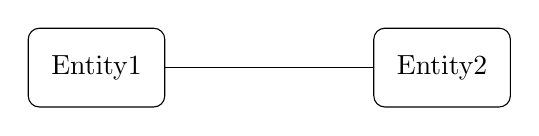
\begin{tikzpicture}
\node[rectangle, rounded corners, text width=1.5cm,  minimum width=1.5cm, minimum height=1cm,text centered, draw=black] (E1) {Entity1};
\node[rectangle, rounded corners, text width=1.5cm,  minimum width=1.5cm, minimum height=1cm,text centered, draw=black] at ([xshift=100pt]E1.east) (E2) {Entity2};
\node[shape=coordinate] at ([xshift=20pt]E1.east) (P1) {};
\node[shape=coordinate] at ([xshift=-20pt]E2.west) (P2) {};
\draw (P1) -- (P2);
\draw (P2) -- (E2.west);
\draw (P1) -- (E1.east);
\end{tikzpicture}

One to Many

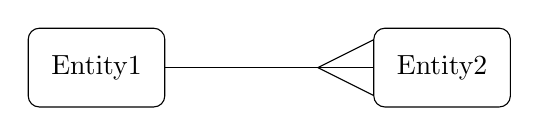
\begin{tikzpicture}
\node[rectangle, rounded corners, text width=1.5cm,  minimum width=1.5cm, minimum height=1cm,text centered, draw=black] (E1) {Entity1};
\node[rectangle, rounded corners, text width=1.5cm,  minimum width=1.5cm, minimum height=1cm,text centered, draw=black] at ([xshift=100pt]E1.east) (E2) {Entity2};
\node[shape=coordinate] at ([xshift=20pt]E1.east) (P1) {};
\node[shape=coordinate] at ([xshift=-20pt]E2.west) (P2) {};
\draw (P1) -- (P2);
\draw (P2) -- (E2.west);
\draw (P2) -- ([yshift=-10pt]E2.west);
\draw (P2) -- ([yshift=10pt]E2.west);
\draw (P1) -- (E1.east);
\end{tikzpicture}

Many to One

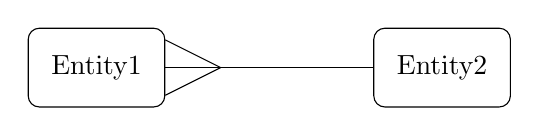
\begin{tikzpicture}
\node[rectangle, rounded corners, text width=1.5cm,  minimum width=1.5cm, minimum height=1cm,text centered, draw=black] (E1) {Entity1};
\node[rectangle, rounded corners, text width=1.5cm,  minimum width=1.5cm, minimum height=1cm,text centered, draw=black] at ([xshift=100pt]E1.east) (E2) {Entity2};
\node[shape=coordinate] at ([xshift=20pt]E1.east) (P1) {};
\node[shape=coordinate] at ([xshift=-20pt]E2.west) (P2) {};
\draw (P1) -- (P2);
\draw (P2) -- (E2.west);
\draw (P1) -- (E1.east);
\draw (P1) -- ([yshift=-10pt]E1.east);
\draw (P1) -- ([yshift=10pt]E1.east);
\end{tikzpicture}

Many to Many

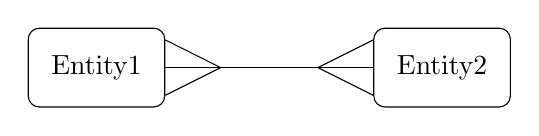
\begin{tikzpicture}
	\node[rectangle, rounded corners, text width=1.5cm,  minimum width=1.5cm, minimum height=1cm,text centered, draw=black] (E1) {Entity1};
	\node[rectangle, rounded corners, text width=1.5cm,  minimum width=1.5cm, minimum height=1cm,text centered, draw=black] at ([xshift=100pt]E1.east) (E2) {Entity2};
	\node[shape=coordinate] at ([xshift=20pt]E1.east) (P1) {};
	\node[shape=coordinate] at ([xshift=-20pt]E2.west) (P2) {};
	\draw (P1) -- (P2);
	\draw (P2) -- (E2.west);
	\draw (P2) -- ([yshift=-10pt]E2.west);
	\draw (P2) -- ([yshift=10pt]E2.west);
	\draw (P1) -- (E1.east);
	\draw (P1) -- ([yshift=-10pt]E1.east);
	\draw (P1) -- ([yshift=10pt]E1.east);
\end{tikzpicture}

If we were to represent the top example using an entity relationship diagram, we would first need to decide how each of the entities are related to one another. We can see that there is no direct relationship between a member and a person, they are only related to each other via rentals. We can see that each member can rent multiple books, so each member can have multiple rentals, but the reverse isn't true, each rental cannot have multiple members, each rental is specific to one of the library members. This means there's a one to many relationship between the members and the rentals. We can also see that each book may be part of multiple rentals, but the reverse isn't true (a rental cannot contain multiple books), so we can say there is a many to one relationship between rentals and books. An entity relationship diagram of this would be as follows:

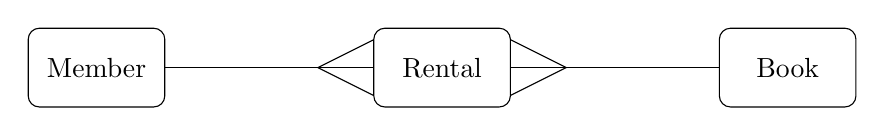
\begin{tikzpicture}
	\node[rectangle, rounded corners, text width=1.5cm,  minimum width=1.5cm, minimum height=1cm,text centered, draw=black] (E1) {Member};
	\node[rectangle, rounded corners, text width=1.5cm,  minimum width=1.5cm, minimum height=1cm,text centered, draw=black] at ([xshift=100pt]E1.east) (E2) {Rental};
	\node[rectangle, rounded corners, text width=1.5cm,  minimum width=1.5cm, minimum height=1cm,text centered, draw=black] at ([xshift=100pt]E2.east) (E3) {Book};
	\node[shape=coordinate] at ([xshift=20pt]E1.east) (P1) {};
	\node[shape=coordinate] at ([xshift=-20pt]E2.west) (P2) {};
	\node[shape=coordinate] at ([xshift=20pt]E2.east) (P3) {};
	\node[shape=coordinate] at ([xshift=-20pt]E3.west) (P4) {};
	\draw (P1) -- (P2);
	\draw (P2) -- (E2.west);
	\draw (P2) -- ([yshift=-10pt]E2.west);
	\draw (P2) -- ([yshift=10pt]E2.west);
	\draw (P1) -- (E1.east);
	\draw (P3) -- (P4);
	\draw (P4) -- (E3.west);
	\draw (P3) -- (E2.east);
	\draw (P3) -- ([yshift=-10pt]E2.east);
	\draw (P3) -- ([yshift=10pt]E2.east);
\end{tikzpicture}

\subsection{Relational databases}

A relational database is a collection of tables which are linked together by means of primary and foreign keys, these are what form the relationship between tables. There are 4 key terms which we need to define:
\begin{itemize}
	\item Attribute
		\subitem A property or characteristics of an entity
	\item Primary Key
		\subitem An attribute which uniquely identifies each record in the table, this is linked to the concept of an Entity identifier, which is an attribute that uniquely identifies each instance of an entity.
	\item Composite Primary Key
		\subitem A set of attributes which uniquely identify each record in a table
	\item Foreign Key
		\subitem An attribute in a table that is a primary key in another table and is used to link tables together.
\end{itemize}

\subsection{Database design and normalisation techniques}

Normalisation is a technique used to produce a normalised set of entities in a database. It is done to make sure that the data within a database is stored efficiently. This involves removing redundant data, and making sure each attribute is atomic (meaning that the attribute can't be broken down further. An example of atomisation is breaking up the attribute \verb|Name| into \verb|forename| and \verb|surnname|). You need to know the third normalised form (3NF), to do this we also need to define first normal form (1NF) and second normal form (2NF).

For our description of normalisation, we will start from the following table:

\begin{table}[H]
	\begin{tabular}{| C{2cm} | C{2.5cm} | C{2.2cm} | C{1.8cm} | C{3cm} |}
		\hline
		StudentID & Name & Teacher & Class & Subject \\\hline
		1 & Nathan Douglas & Ms. Maharaj, Mrs. Ozgu, Mr. Hamshar & R1,R2,R3 & English, Chemistry, Maths \\\hline
		2 & Helen Douglas & Mrs. Maharaj, Mr. Johnston, Mrs. Read & R1,R4,R5 & English, Biology, History \\\hline
		3 & Ryan Potter & Mr. Hamshar, Mr. Hillary, Mr. Johnston & R3, R6, R4 & Maths, Physics, Biology \\\hline
	\end{tabular}
\end{table}

First Normal Form (1NF) - This involves making sure each attribute is atomic (can no longer be broken down further) and only a single value is entered in each attribute (all data in the table is atomic). So to convert our table to first normal form, we would get:

\begin{table}[H]
	\begin{tabular}{| l | l | l | l | l | l |}
		\hline
		StudentID & Forename & Surname & Teacher & Class & Subject \\\hline
		1 & Nathan & Douglas & Ms. Maharaj & R1 & English \\\hline
		1 & Nathan & Douglas & Mrs. Ozgu & R2 & Chemistry \\\hline
		1 & Nathan & Douglas & Mr. Hamshar & R3 & Maths \\\hline
		2 & Helen & Douglas & Ms. Maharaj & R1 & English \\\hline
		2 & Helen & Douglas & Mr. Johnston & R4 & Biology \\\hline
		2 & Helen & Douglas & Mrs. Read & R5 & History \\\hline
		3 & Ryan & Potter & Mr. Hamshar & R3 & Maths \\\hline
		3 & Ryan & Potter & Mr. Hillary & R6 & Physics \\\hline
		3 & Ryan & Potter & Mr. Johnston & R4 & Biology \\\hline
	\end{tabular}
\end{table}

So we have broken down the name attribute into forename and surname, we have also made sure that all of the data is atomic, creating new records to make sure this is the case.

Second Normal Form (2NF) - This is achieved by first making sure the table is in first normal form, and then removing attributes that only partially depend on the key by creating new tables. So for example, the process of converting from 1NF to 2NF may be as follows

\begin{table}[H]
	\begin{tabular}{| l | l | l | l |}
		\hline
		StudentID & Forename & Surname & TeacherID\\\hline
		1 & Nathan & Douglas & 1\\\hline
		1 & Nathan & Douglas & 2\\\hline
		1 & Nathan & Douglas & 3\\\hline
		2 & Helen & Douglas & 1\\\hline
		2 & Helen & Douglas & 4\\\hline
		2 & Helen & Douglas & 5\\\hline
		3 & Ryan & Potter & 3\\\hline
		3 & Ryan & Potter & 6\\\hline
		3 & Ryan & Potter & 4\\\hline
	\end{tabular}
	
	\begin{tabular}{| l | l | l | l |}
		\hline
		TeacherID & Teacher & Class & Subject \\\hline
		1 & Ms. Maharaj & R1 & English \\\hline
		2 & Mrs. Ozgu & R2 & Chemistry \\\hline
		3 & Mr. Hamshar & R3 & Maths \\\hline
		4 & Mr. Johnston & R4 & Biology \\\hline
		5 & Mrs. Read & R5 & History \\\hline
		6 & Mr. Hillary & R6 & Physics \\\hline
	\end{tabular}
\end{table}

This first table is still not in 2NF as a composite key of StudentID and TeacherID would be needed, however then Forename and Surname only depend on StudentID, thus it needs to be broken down further, thus we will need to create a new table to split this up again, obtaining:

\begin{table}[H]
	\begin{tabular}{| l | l | l |}
		\hline
		StudentID & Forename & Surname \\\hline
		1 & Nathan & Douglas\\\hline
		2 & Helen & Douglas\\\hline
		3 & Ryan & Potter\\\hline
	\end{tabular}
	
	\begin{tabular}{| l | l |}
		\hline
		StudentID & TeacherID\\\hline
		1 & 1\\\hline
		1 & 2\\\hline
		1 & 3\\\hline
		2 & 1\\\hline
		2 & 4\\\hline
		2 & 5\\\hline
		3 & 3\\\hline
		3 & 6\\\hline
		3 & 4\\\hline
	\end{tabular}
	
	\begin{tabular}{| l | l | l | l |}
		\hline
		TeacherID & Teacher & Class & Subject \\\hline
		1 & Ms. Maharaj & R1 & English \\\hline
		2 & Mrs. Ozgu & R2 & Chemistry \\\hline
		3 & Mr. Hamshar & R3 & Maths \\\hline
		4 & Mr. Johnston & R4 & Biology \\\hline
		5 & Mrs. Read & R5 & History \\\hline
		6 & Mr. Hillary & R6 & Physics \\\hline
	\end{tabular}
\end{table}

So we have now broken the first table down into 2 tables where all of the data is entirely dependant on the primary key, and now the whole database is in 2NF.

Third Normal Form (3NF) - The database must be in second normal form, and then all non-key attributes that are dependant on other non-key attributes are removed via creation of a new table. In the above example, this means we will get rid of the subject attribute as it depends on class, and then create a new table containing class and subject:

\begin{table}[H]
	\textbf{Student}
	
	\begin{tabular}{| l | l | l |}
		\hline
		StudentID & Forename & Surname \\\hline
		1 & Nathan & Douglas\\\hline
		2 & Helen & Douglas\\\hline
		3 & Ryan & Potter\\\hline
	\end{tabular}
	
	\vspace{0.5cm}
	
	\textbf{StudentTeacher}
	
	\begin{tabular}{| l | l |}
		\hline
		StudentID & TeacherID\\\hline
		1 & 1\\\hline
		1 & 2\\\hline
		1 & 3\\\hline
		2 & 1\\\hline
		2 & 4\\\hline
		2 & 5\\\hline
		3 & 3\\\hline
		3 & 6\\\hline
		3 & 4\\\hline
	\end{tabular}
	
	\vspace{0.5cm}
	
	\textbf{Teacher}
	
	\begin{tabular}{| l | l | l |}
		\hline
		TeacherID & Teacher & Class \\\hline
		1 & Ms. Maharaj & R1 \\\hline
		2 & Mrs. Ozgu & R2 \\\hline
		3 & Mr. Hamshar & R3 \\\hline
		4 & Mr. Johnston & R4 \\\hline
		5 & Mrs. Read & R5 \\\hline
		6 & Mr. Hillary & R6 \\\hline
	\end{tabular}
	
	\vspace{0.5cm}
	
	\textbf{Subject}
	
	\begin{tabular}{| l | l |}
		\hline
		Class & Subject \\\hline
		R1 & English \\\hline
		R2 & Chemistry \\\hline
		R3 & Maths \\\hline
		R4 & Biology \\\hline
		R5 & History \\\hline
		R6 & Physics \\\hline
	\end{tabular}
\end{table}

\subsection{Structured Query Language (SQL)}

There are 5 things you need to be able to do in SQL

Retrieve Data

This is used to query a database, and easily get data from inside a database, the query is often of the current form:
\begin{verbatim}
SELECT FieldName1, FieldName2, FieldName3, ...
FROM Table1, Table2, Table3, ...
WHERE Condition,
ORDER BY FieldName DESC/ASC;
\end{verbatim}

You can easily view a whole table by using the following form:

\begin{verbatim}
SELECT * FROM Table;
\end{verbatim}

So for example, if we wanted to find all the Subjects that Nathan Douglas had, we could use

\begin{verbatim}
SELECT Student.Forename, Student.Surname, Subject.Subject
FROM Student, StudentTeacher, Teacher, Subject
WHERE Student.Forename = "Nathan" AND Student.Surname = "Douglas" AND Student.StudentID = Student.StudentID = StudentTeacher.StudentID AND StudentTeacher.TeacherID = Teacher.TeacherID AND Teacher.Class = Subject.Class
ORDER BY Subject.Subject ASC;
\end{verbatim}

and it would return:

\begin{table}[H]
	\begin{tabular}{| l | l | l |}\hline
		Forename & Surname & Subject \\\hline
		Nathan & Douglas & Chemistry \\\hline
		Nathan & Douglas & English \\\hline
		Nathan & Douglas & Maths \\\hline
	\end{tabular}
\end{table}

Here are all of the boolean comparators you should know:

\begin{table}[H]
	\begin{tabular}{| l | L{8cm} | l |}\hline
		Operator 	& Description 								& Example \\\hline
		= 			& Equal 									& \verb|Name = `Bob'| \\\hline
		<> 			& Not Equal									& \verb|Income <> 0| \\\hline
		> 			& Greater Than 								& \verb|Height > 1.4| \\\hline
		< 			& Less Than 								& \verb|Weight < 100| \\\hline
		>= 			& Greater Than or Equal To 					& \verb|Age >= 18| \\\hline
		<= 			& Less Than or Equal To 					& \verb|Temperature <= 25| \\\hline
		BETWEEN 	& Between an Inclusive range 				& \verb|Cousins BETWEEN 1 and 7| \\\hline
		LIKE 		& Search for a Pattern (\verb|%| equivalent to  .* regex, \verb|_| equivalent to . regex)	& \verb|Name LIKE `%oh_'| \\\hline
		IN 			& Specify multiple possible values of a row	& \verb|Siblings IN (1,2,3)| \\\hline
	\end{tabular}
\end{table}

(If you want to be snazzy, you could teach yourself about inner joins, which can make queries above shorter and easier to read, but they aren't necessary so...)

Update Data

This is used to change data that is already present in a table, the general format for this sort of SQL is

\begin{verbatim}
UPDATE Table
SET FieldName1 = value1, FieldName2 = value2, ...
WHERE Condition;
\end{verbatim}

for example, if we wanted to change Nathan Douglas's Name to Wally West, I would write the following SQL statement:

\begin{verbatim}
UPDATE Student
SET Forename = 'Wally', Surname = 'West'
WHERE Forename = 'Nathan';
\end{verbatim}

Insert Data

This is used to insert data into an existing table, if you want to insert data into specific columns (leaving the others null, or letting them be auto-completed via the set-up of the table), you would use the following

\begin{verbatim}
INSERT INTO Table (FieldName1, FieldName2, FieldName3, ...)
VALUES (value1, value2, value3, ...);
\end{verbatim}

If you want to insert into all of the columns in a table, you can use the above, or the following

\begin{verbatim}
INSERT INTO Table
VALUES (value1, value2, value3, ...);
\end{verbatim}

If I wanted to add a new student into the database with StudentID of 4 called Anik Roy, I would write the following statement:

\begin{verbatim}
INSERT INTO Student
VALUES (1, Anik, Roy);
\end{verbatim}

Delete Data

This is used to delete records within a table, it has general form:

\begin{verbatim}
DELETE FROM Table
WHERE Condition;
\end{verbatim}

To delete all the records in a table, we can use:

\begin{verbatim}
DELETE FROM Table
\end{verbatim}

So if we wanted to delete Helen Douglas from the Student table, we would write the following:

\begin{verbatim}
DELETE FROM Student
WHERE Forename = 'Helen' AND Surname = 'Douglas';
\end{verbatim}

Create Table

To add a table to a data base we can use the following form:

\begin{verbatim}
CREATE TABLE Table (
	FieldName1 datatype,
	FieldName2 datatype,
	FieldName3 datatype,
	...
);
\end{verbatim}

A list of common data types are:

\begin{table}[H]
	\begin{tabular}{| l | l |}\hline
		character(n) & A string of fixed length n\\\hline
		varchar(n) & A string of variable length less than or equal to n\\\hline
		boolean & True or False\\\hline
		int & Any integer (positive or negative whole number)\\\hline
		decimal(p,s) & A decimal number of  length p , and s digits after the decimal point\\\hline
		real & Any real number\\\hline
		date & The date (format \verb|DATE`YYYY-MM-DD'|)\\\hline
		time & The time (format \verb|TIME`HH-MM-SS'|)\\\hline
	\end{tabular}
\end{table}

To create the Student table, I would write the following statement:

\begin{verbatim}
CREATE TABLE Student (
	StudentID int AUTO_INCREMENT,
	Forename varchar(255),
	Surname varchar(255),
	PRIMARY KEY (StudentID)
);
\end{verbatim}

The \verb|AUTO_INCREMENT| means that the StudentID does not need to be inputted every time a new set of data is added, and the \verb|PRIMARY KEY (StudentID)| sets StudentID as the primary key.

\subsection{Client server databases}

Within some projects involving more than one person, multiple people may need to be able to access and edit the database. A way to implement this is to use a client-server database, where the database is hosted on a server that different users can access, all processing is then done on this main server.

When working with this sort of database, we need to take into account what may occur if two people were to access and update the same piece of data at the same time (concurrently). If the situation isn't dealt with properly, this could lead to loss of data, as the data from one user could be overwritten by another user, but the first users data may be more accurate. There are 4 main ways to deal with concurrent access:
\begin{itemize}
	\item Record Lock
		\subitem For this, you just only allow one user at a time to edit a record, and lock the record for other users.  This means that the first user is able to read and write data, whereas anyone else can only read data, until the first user is done.
	\item Serialisation
		\subitem For this, we allow multiple users to edit the database at the same time, however if a user updates the database, all of the other users are forced to restart, and are thus presented with an up to date database. This means that only one action occurs at a time.
	\item Timestamp ordering
		\subitem This is a way to order the commands so that they can be serialised. Whenever a user accesses a database they are given a timestamp (which can just be represented by an incremented integer). To be able to write to the database, you must have timestamp later than the latest read or write transaction. To be able to read from the database you must have timestamp later than the latest write transaction.
	\item Commitment ordering
		\subitem In this, the transactions are created on the device, and then sent to the server to be scheduled, depending on the commands within the transaction and the time which the transaction occurred.
\end{itemize}